\documentclass[14pt]{beamer}
\usetheme{Warsaw}
\usecolortheme{beaver}
\usefonttheme{professionalfonts}

\input{../../preamble}
\usepackage{amscd,amsmath,amssymb,amsthm,graphicx}
\usepackage{paralist}
\usepackage{tabto}
\usepackage[normalem]{ulem}
\usepackage{tikz}
\usepackage{tkz-euclide}
\usetkzobj{all}

% % % % % % % % % %
\title[Cal I S2015]{MATH 2554 (Calculus I)}
\subtitle{}
\author[Wheeler]{Dr. Ashley K. Wheeler}
\institute{University of Arkansas}
\date{\today}
\logo{}

% % %
\begin{document}
\maketitle

% % %
\begin{frame}
\frametitle{Table of Contents}
\tableofcontents
\end{frame}

% % % % % % % % % % Mon 6 Apr 2015

% % %
\begin{frame}
\section[Week 12]{Week 12: 6-10 April}
\frametitle{Monday 6 April (Week 1w)}
\small
\begin{itemize}
\item Exam \#3: Is now a Take Home.  Due Friday in class.
\item Computer HW this week: $\oint 4.6-4.7$ 	
\item Quiz \#11 Thurs 9 April Take Home covers $\oint 4.6-4.7$ .
\item next week: Quiz \#12 In Class ($\oint 5.1$ and $\Sigma$ notation) Thurs 16 April, then Quiz \#13 ($\oint 4.8, 5.1, 5.2$) Take Home due Tues 20 Apr
\end{itemize}
\end{frame}

% % %
\begin{frame}
\subsection[$\oint 4.5$ Linear Approximation and Differentials]{$\oint 4.5$ Linear Approximation and Differentials}
\frametitle{$\oint 4.5$ Linear Approximation and Differentials}
\footnotesize
Suppose $f$ is a function such that $f^{\prime}$ exists at some point $P$.  If you zoom in on the graph, the curve appears more and more like the tangent line to $f$ at $P$.  

\centering{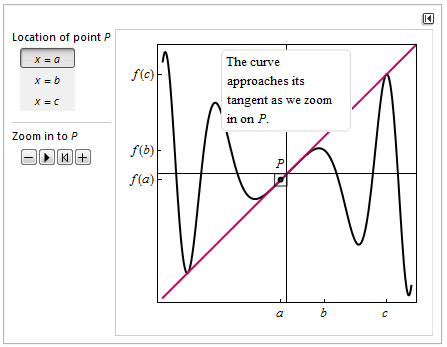
\includegraphics[scale=0.54]{linApprox}}
\end{frame}

% % %
\begin{frame}
\frametitle{\small Linear Approximation}
\footnotesize
This idea -- that \alert{smooth} curves (i.e., curves without corners) appear straighter on smaller scales -- is the basis of linear approximations.

\vspace{1pc}
One of the properties of a function that is \alert{differentiable} at a point $P$ is that it is \alert{locally linear} near $P$ (i.e., the curve approaches the tangent line at $P$.)

\vspace{1pc}
Therefore, it makes sense to approximate a function with its tangent line, which matches the value and slope of the function at $P$.  

\vspace{1pc}
This is why you've had to do so many ``find the equation for the tangent line to the given point" problems!
\end{frame}

% % %
\begin{frame}
\frametitle{}
\footnotesize
\begin{dfn} Suppose $f$ is differentiable on an interval $I$ containing the point $a$.  The {\bf linear approximation} to $f$ at $a$ is the linear function
\[L(x)=f(a)+f^{\prime}(a)(x-a)\qquad\text{for $x$ in $I$.}\]
\end{dfn}

\vspace{1pc}
{\bf Remarks:} Compare this definition to the following: At a given point $P=(a,f(a))$, the slope of the line tangent to the curve at $P$ is $f^{\prime}(a)$.  So the equation of the tangent line is
\[y-f(a)=f^{\prime}(a)(x-a).\]

(Yes, it is the same thing!)
\end{frame}

% % %
\begin{frame}
\frametitle{}
\small
\begin{exe} Write the equation of the line that represents the linear approximation to 
\[f(x)=\dfrac{x}{x+1}\qquad\text{ at $a=1$.}\]  
Then {\it use} the linear approximation to estimate $f(1.1)$. \end{exe}

\vspace{1pc}
{\bf Solution:} First compute
\[f^{\prime}(x)=\dfrac{1}{(x+1)^2},\quad f(a)=\dfrac{1}{2},\quad f^{\prime}(a)=\dfrac{1}{4}\]
\[L(x)=\dfrac{1}{2}+\dfrac{1}{4}(x-1)=\dfrac{1}{4}x+\dfrac{1}{4}.\]
\end{frame}

% % %
\begin{frame}
\small
{\bf Solution (continued):}

\bigskip

Because $x=1.1$ is near $a=1$, we can estimate $f(1.1)$ using $L(1.1)$:
$$f(1.1) \approx L(1.1)= 0.525$$

\bigskip

Note that $f(1.1)=0.5238$, so the error in this estimation is
$$\dfrac{0.525-0.5238}{0.5238} \times 100=0.23 \%.$$
\end{frame}

% % %
\begin{frame}
\frametitle{\small Intro to Differentials}
\small
Our linear approximation $L(x)$ is used to approximate $f(x)$ when $a$ is fixed and $x$ is a nearby point:
\[f(x) \approx f(a)+f^{\prime}(a)(x-a)\]

\vspace{1pc}
When rewritten,
\begin{align*}
f(x)-f(a) & \approx f^{\prime}(a)(x-a) \\[0.5pc]
\implies \Delta y & \approx f^{\prime}(a) \Delta x.
\end{align*}
\end{frame}

% % %
\begin{frame}
\footnotesize
A change in $y$ can be approximated by the corresponding change in $x$, magnified or diminished by a factor of $f^{\prime}(a)$.  

\vspace{1pc}
This is another way to say that $f^{\prime}(a)$ is the rate of change of $y$ with respect to $x$!
\begin{align*}
\Delta y & \approx f^{\prime}(a) \Delta x \\[0.5pc]
\frac{\Delta y}{\Delta x} & \approx f^{\prime}(a)
\end{align*}

\vspace{1pc}
So if $f$ is differentiable on an interval $I$ containing the point $a$, then the change in the value of $f$ (the $\Delta y$), between two points $a$ and $a+\Delta x$ in $I$, is \alert{approximately} $f'(x)\Delta x$. 
\end{frame}

% % %
\begin{frame}
\small
We now have two different, but related quantities:

\begin{itemize}
\item The change in the function $y=f(x)$ as $x$ changes from $a$ to $a+\Delta x$ (which we call $\Delta y$).

\vspace{0.5pc}
\item The change in the linear approximation $y=L(x)$ as $x$ changes from $a$ to $a+\Delta x$ (called the \alert{differential}, $dy$).
\end{itemize}

%\vspace{0.5pc}
\[\Delta y \approx dy\]
\end{frame}

% % %
\begin{frame}
\frametitle{}
\small
When the $x$-coordinate changes from $a$ to $a+\Delta x$:
\begin{itemize}
\item The function change is \underline{{\bf exactly}} $\Delta y=f(a+\Delta x)-f(a)$.
\item The linear approximation change is 
\begin{alignat*}{2}
\Delta L &= L(a+\Delta x)-L(a) \\[0.5pc]
&= \left( f(a)+f^{\prime}(a)(a+\Delta x -a) \right) - \left( f(a)+f^{\prime}(a)(a-a) \right) \\[0.5pc]
&= f^{\prime}(a) \Delta x
\end{alignat*}
and this is $dy$.
\end{itemize}
\end{frame}

% % %
\begin{frame}
\small
We define the differentials $dx$ and $dy$ to distinguish between the \alert{change in the function ($\Delta y$)} and the \alert{change in the linear approximation ($\Delta L$)}: 
\begin{itemize}
\item $dx$ is simply the change in $x$, i.e.\ $\Delta x$.
%\vspace{0.25pc}
\item $dy$ is the change in the linear approximation, which is $\Delta L=f^{\prime}(a) \Delta x$.
\end{itemize}

{\bf SO:}
\begin{align*}
\Delta L &= f^{\prime}(a) \Delta x \\[0.5pc]
dy &= f^{\prime}(a) dx \\[0.5pc]
\dfrac{dy}{dx} &= f^{\prime}(a)\quad \text{ (at $x=a$)}
\end{align*}
\end{frame}

% % %
\begin{frame}
\frametitle{}
\small
\begin{dfn} Let $f$ be differentiable on an interval containing $x$.
\begin{itemize}
\item A small change in $x$ is denoted by the {\bf differential} $dx$.
\item The corresponding change in $y=f(x)$ is \underline{approximated} by the {\bf differential} $dy=f^{\prime}(x)dx$; that is,
\begin{align*}
\Delta y& = f(x+\Delta x)-f(x) \\[0.5pc]
\approx dy &= f^{\prime}(x)dx.
\end{align*}
\end{itemize}
\end{dfn}

\vspace{1pc}
{\bf The use of differentials is critical as we approach integration.}
\end{frame}

% % %
\begin{frame}
\frametitle{}
\small
\begin{ex} Use the notation of differentials $[dy = f^{\prime}(x) dx]$ to approximate the change in $f(x)=x-x^3$ given a small change $dx$. \end{ex}

{\bf Solution:}

$f^{\prime}(x)=1-3x^2$, so $dy=(1-3x^2)dx.$

A small change $dx$ in the variable $x$ produces an approximate change of $dy=(1-3x^2)dx$ in $y$.

\vspace{1.5pc}
For example, if $x$ increases from 2 to 2.1, then $dx=0.1$ and 
\[dy=\left(1-3(2)^2 \right)(0.1)=-1.1.\]
This means as $x$ increases by 0.1, $y$ decreases by 1.1.
\end{frame}

% % %
\begin{frame}
\frametitle{HW from Section 4.5}
Do problems 7--9 all, 11, 12, 29--38 all (p.\ 273 in textbook)
\end{frame}


% % % % % % % % % % Wed 1 Apr 2015

% % %
\begin{frame}
\frametitle{Wednesday 1 April (Week 11)}
\small
\begin{itemize}
\item Computer HW this week: $\oint 4.4-4.5$
\item Exam \#3 Friday 3 April -- up to $\oint 4.5$
\item Quiz \#11 Take Home given Thurs 9 Apr covers $\oint 4.6-4.7$
\item today: Review for Exam 3
\end{itemize}
\end{frame}

% % %
\begin{frame}
\frametitle{\small 3.8 Derivatives of Logarithmic and Exponential Functions}
\small
\begin{itemize}
\item Be able to compute derivatives involving $\ln x$ and $\log_b x$
\item Be able to compute derivatives of exponential functions of the form $b^x$
\item Be able to use logarithmic differentiation to determine $f^{\prime}(x)$
\end{itemize}
\end{frame}

% % %
\begin{frame}
\frametitle{\small 3.9 Derivatives of Inverse Trig Functions}
\small
\begin{itemize}
\item Know the derivatives of the six inverse trig functions.
\item Also: You are responsible for every derivative rule and every derivative formula we have covered this semester.
\end{itemize} 
\end{frame}

% % %
\begin{frame}
\frametitle{\small 3.10 Related Rates}
\small
\begin{itemize}
\item Know the steps to solving related rates problems, and be able to use them to solve problems given variables and rates of change.
\item Be able to solve related rates problems.  If, while doing the HW (paper or computer), you were provided a formula in order to solve the problem, then I will do the same.  If you were not provided a formula while doing the HW (paper or computer), then I also will not provide the formula.
\end{itemize}
\end{frame}

% % %
\begin{frame}
\frametitle{\small 4.1 Maxima and Minima}
\small
\begin{itemize}
\item Know the definitions of maxima, minima, and what makes these points local or absolute extrema (both analytically and graphically).
\item Know how to find critical points for a function.
\item Given a function on a given interval, be able to find local and/or absolute extrema.
\item Given specified properties of a function, be able to sketch a graph of that function.
\end{itemize}
\end{frame}

% % %
\begin{frame}
\frametitle{\small 4.2 What Derivatives Tell Us}
\footnotesize
\begin{itemize}
\item Be able to use the first derivative to determine where a function is increasing or decreasing.
\item Be able to use the \alert{First Derivative Test to identify local maxima and minima}.  Be able to explain in words how you arrived at your conclusion.
\item Be able to find critical points, absolute extrema, and inflection points for a function.
\item Be able to use the second derivative to determine the concavity of a function.
\item Be able to use the \alert{Second Derivative Test to determine whether a given point is a local max or min}.  Be able to explain in words how you arrived at your conclusion.
\item Know your Derivative Properties!!! (see Figure 4.36 on p.\ 242)
\end{itemize}
\end{frame}

% % %
\begin{frame}
\frametitle{\small 4.3 Graphing Functions}
\small
\begin{itemize}
\item Be able to find specific characteristics of a function that are spelled out in the Graphing Guidelines on p.\ 248 (e.g., know how to find $x$- and $y$-intercepts, vertical/horizontal asymptotes, critical points, inflection points, intervals of concavity and increasing/decreasing, etc.).  
\item Be able to use these specific characteristics of a function to sketch a graph of the function.
\item TIP: If you are looking for intervals for increasing/decreasing or concave up/down, you should {\it treat} the naughty points as critical points and/or possible points of inflection.
\end{itemize} 
\end{frame}

% % %
\begin{frame}
\frametitle{\small 4.4 Optimization Problems}
\small
\begin{itemize}
\item Be able to solve optimization problems that maximize or minimize a given quantity.
\item Be able to identify and express the constraints and objective function in an optimization problem.
\item Be able to determine your interval of interest in an optimization problem (e.g., what range of $x$-values are you searching for your extreme points?)
\item {\bf As to formulas, the same comment made above with respect to formulas for related rates problems applies here as well.}
\end{itemize}
\end{frame}

% % %
\begin{frame}
\frametitle{\small 4.5 Linear Approximation and Differentials}
\small
\begin{itemize}
\item Be able to find a linear approximation for a given function.
\item Be able to use a linear approximation to estimate the value of a function at a given point.
\item Be able to use differentials to express how the change in $x$ ($dx$) impacts the change in $y$ ($dy$).
\end{itemize}
\end{frame}


% % %
\begin{frame}
\frametitle{Pep Talk}
\footnotesize
\begin{itemize}
\item one $3\times 5$ inch notecard, one-sided only
\item Read the question!  
\item Do the book problems.
\item Find a buddy who understands concepts a little better than you and work on problems for 2-3 hours.  Then find a buddy who is struggling and work with them 2-3 hours.  Explaining to someone else tests how deeply you really know the material.  This strategy also helps reduce stress because it doesn't require you to devote a full day or night of studying, just 2-3 hours at a time of productive work.
\end{itemize}
\end{frame}

% % %
\begin{frame}
\frametitle{Running out of Time on the Exam, cont.}
\footnotesize
\begin{itemize}
\item If you encounter an unfamiliar type of problem on the exam, relax, because it's most likely not a trick.  The solutions will always rely on the information from the required reading/assignments.  Take your time and do each baby step carefully.  
\item During the exam, do the problems you are most confident with first!  Different people will find different problems easier.
\item The exam is not a race.  If you finish early take advantage of the time to check your work.  You don't want to leave feeling smug about how quickly you finished only to find out next week you lost a letter grade's worth of points from silly mistakes.
\item Algebra: Look at solutions to Quiz 10 (and others).
\end{itemize}
\end{frame}

\begin{comment}
\end{comment}

\end{document}